\section{Conjuntos de Datos y Configuración Experimental}

\subsection{Datasets Geoespaciales}

Resulta revelador observar cómo la selección de datasets influye de manera decisiva en las conclusiones que pueden extraerse en tareas de compresión geoespacial. Molliere et al. \cite{Molliere2025_Learned_EO_Compression} destacan en su trabajo la importancia de utilizar imágenes representativas de misiones reales para evaluar learned compression en Earth Observation.

En este estudio se emplearon principalmente tres fuentes complementarias: imágenes Sentinel-2 (multiespectral), escenas Landsat-9 y un conjunto de imágenes hiperespectrales de la misión PRISMA. Se priorizaron regiones con alta variabilidad: zonas urbanas densas, áreas agrícolas extensas, bosques tropicales y regiones áridas, todas relevantes para aplicaciones de exploración.

\begin{table*}[h]
\centering
\caption{Estadísticas de los conjuntos de datos utilizados}
\label{tab:estadisticas_datasets}
\begin{tabular}{lcccc}
\hline
\textbf{Dataset} & \textbf{Imágenes} & \textbf{Bandas} & \textbf{Resolución} & \textbf{Uso} \\
\hline
Sentinel-2 MSI & 1850 & 13 & 10-60 m & Entrenamiento principal \\
Landsat-9 OLI & 920 & 11 & 15-30 m & Validación \\
PRISMA Hyper & 450 & 239 & 30 m & Evaluación hiperespectral \\
\hline
\end{tabular}
\end{table*}

Aunque el volumen de datos es sustancial, cabe matizar que la diversidad geográfica y temporal sigue siendo más crítica que la mera cantidad de muestras.

\subsection{Preprocesamiento y Augmentación}

Uno de los desafíos persistentes al trabajar con datos satelitales reales radica en las diferencias de calibración entre sensores y en las degradaciones naturales presentes. Siguiendo aproximaciones similares a las reportadas por Wang et al. \cite{Wang2025_RS_Compression}, se aplicó un pipeline riguroso que incluye corrección radiométrica, recorte en patches no solapados de 256×256 píxeles y normalización por banda.

El preprocesamiento contempló además la eliminación de nubes y sombras mediante máscaras SCL y QA. Para mejorar la robustez del modelo, se implementó una estrategia de augmentación extensa que incluye rotaciones, flips, ajustes de brillo/contraste, simulaciones de ruido atmosférico y variaciones en la resolución efectiva.

\subsection{Métricas Rate-Distortion y Downstream}

Lejos de limitarse a métricas tradicionales, la evaluación buscó reflejar la utilidad real de los datos comprimidos en contextos de exploración. Se calcularon PSNR, MS-SSIM y Learned Perceptual Image Patch Similarity (LPIPS) como indicadores de fidelidad. El rendimiento de compresión se midió principalmente mediante BD-Rate respecto al estándar VTM.

Más relevante aún fue la evaluación en tareas downstream: clasificación de cobertura terrestre con ResNet-50 y detección de anomalías mediante autoencoders. Se midió el impacto de diferentes tasas de compresión en precisión, recall y F1-score.

\begin{figure}[h]
\centering
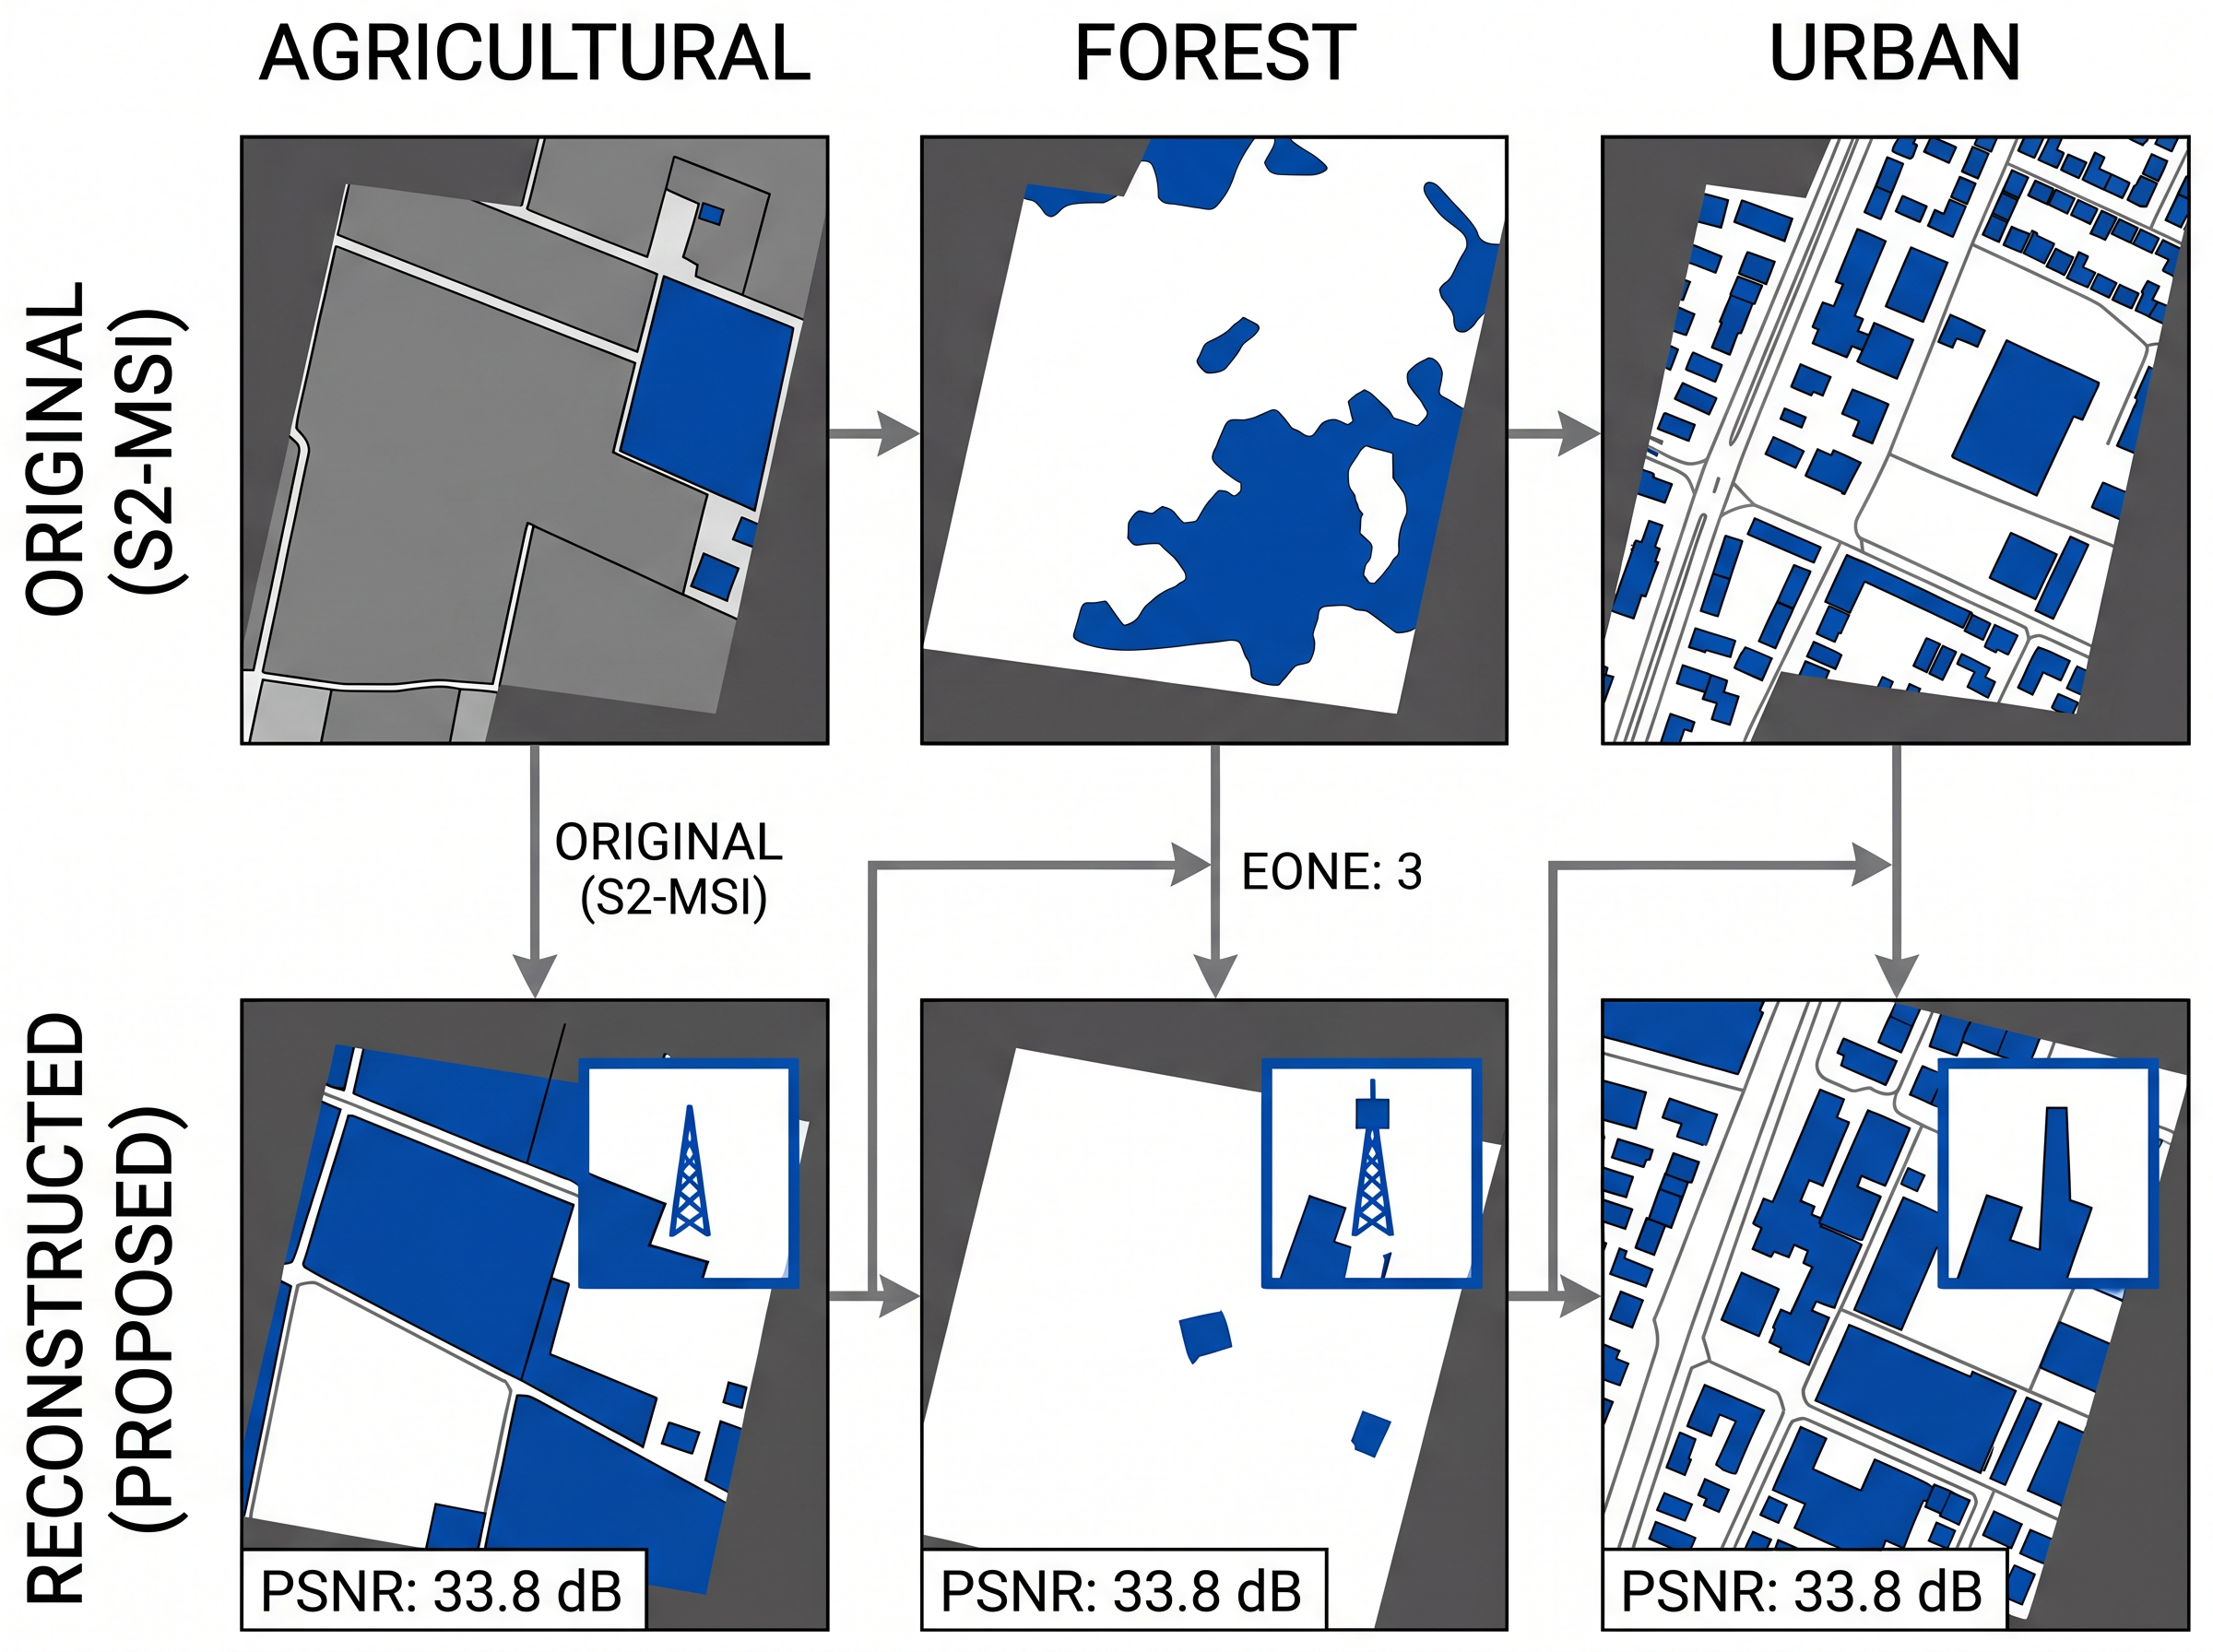
\includegraphics[width=\linewidth]{fig4.png}
\caption{Ejemplos representativos de imágenes originales y reconstruidas a diferentes tasas de compresión. Se muestran parches de Sentinel-2 con énfasis en regiones de interés para exploración (áreas agrícolas, vegetación y zonas urbanas).}
\label{fig:ejemplos_original_reconstruidas}
\end{figure}

Aunque las métricas rate-distortion tienden a correlacionar con la calidad visual, en muchos casos estudiados no capturan completamente la preservación de características semánticas. Esta desconexión justifica precisamente la evaluación integral que se presenta en la siguiente sección.